\documentclass[11pt]{article}
\usepackage[margin=1cm]{geometry}
\usepackage[T1]{fontenc}
\pagenumbering{gobble}
\usepackage{graphicx}
\graphicspath{{img/}}

\title{\vspace*{-1cm}Assembler, Extension and Group Reflection}
\author{\vspace*{-0.1cm}Bartłomiej Cieślar, Jordan Hall, Oliver Killane and Ioana Mihăilescu}
\date{\vspace*{-0.15cm}18 June 2021}

\begin{document}
\maketitle

\section{Introduction}
As the emulator and assembler are separate programs that can be tested and implemented independently, we have made a group decision to complete them in parallel. This report will omit the base implementation of the emulator, because it has already been mentioned in the checkpoint report. The workload was split as follows:
\begin{center}
	\begin{tabular}{ r | l }
		\textbf{Emulator} & \textbf{Assembler} \\
		Ioana \& Oliver & Bartłomiej \& Jordan
	\end{tabular}
\end{center}
\section{Assembler}
\subsection*{Workflow}
The development cycle for the assembler was very simmilar to that of the emulator:\\\\
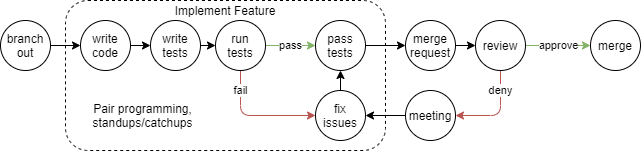
\includegraphics[width = \textwidth]{development_cycle}
In addition, the workload of the assembler was split as follows:\\
\begin{center}
	\begin{tabular}{r|l}
		\textbf{Person Responsible} & \textbf{Feature} \\\
		Bartek & stddata library \\
		Jordan & main data flow \\
		Jordan & tokenizer \\
		Bartek & command processing \\
	\end{tabular}
\end{center}
\subsection*{StdData}
The stddata library, inspired by C++'s STL, has proved invaluable in the implementation of the assembler, although has not been utilized in the emulator. The library features the following structures, the interface of which mimics that of the stl library (with accommodations to the lack of some featues in C):
\begin{itemize}
\item Stack (unused) - an implementation of a vector-based stack
\item Queue (unused) - an implementation of a list-based queue
\item Deque (unused) - an implementation of a list-based deque
\item Vector - a resizable array with static time operations
\item VectorIterator - an iterator for looping over the elements of a vector
\item List - a linked list implementation
\item ListIterator - an iterator for looping over the elements of a list
\item Set - a hashset implementation with buckets implemented using linear probing
\item SetIterator - an iterator for looping over the elements of a set
\item Map - a hashmap implementation with buckets implemented using linear probing
\item MapIterator - an iterator for looping over the elements of a map
\item DecisionTree - a custom data structure similar to a trie working as a map with keys as sequences of items
\end{itemize}
The full documentation of this library (generated using doxygen) can be accessed under lib/stddata/doc/refman.pdf
\subsection*{Data Flow}
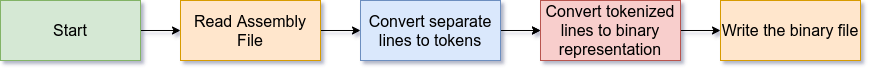
\includegraphics[scale=0.6]{assembler_dataflow}
\subsection*{Tokenization}
The tokenizer is a finite state machine (FSM) that follows the state transition diagram below:
\begin{center}
	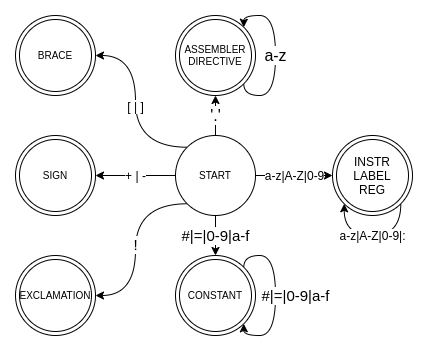
\includegraphics[scale=0.6]{fsmDiagram}
\end{center}
The finite state machine interprets each line character-by-character, and changes its state depending on the above diagram. Single circles are intermediate states, where a token can't be produced if the line ends on that token. Double-circles are the end states, and a token is produced when an end state is reached. The tokenizer does not produce any tokens for lines that have assembler directives on them, and instead will produce directly the desired result of said directive.
The choice to make the tokenizer a finite state machine was most beneficial, allowing us to easily show the correctness of our tokenizer graphically and separate the logic of each state to make the code more readable and easily debug-able.  
\subsection*{Command Generation}
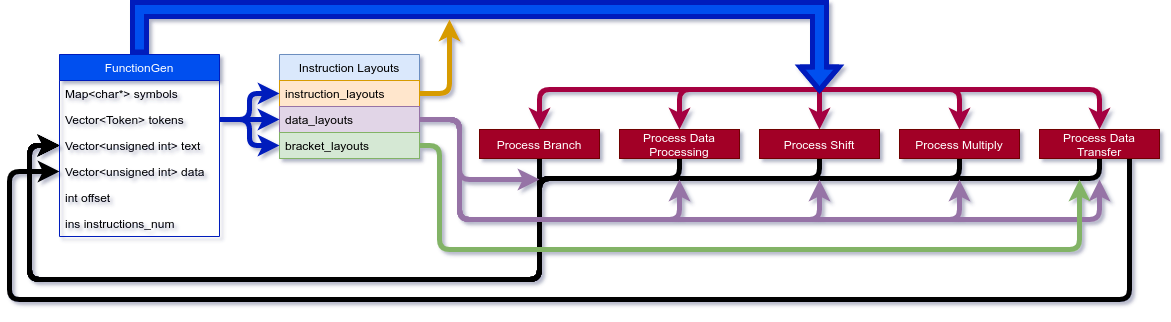
\includegraphics[width=\textwidth]{commandgen}
The command generation consist of 2 stages: processing function dispatch and data conversion to a binary representation. The processing function dispatch uses the sequence of the tokens and a decision tree to determine the appropriate function for the sequence. Then, now inside the processing funciton, it uses another decision tree to determine which fields inside the function need to be set according to which tokens. Since the fields can be set to some values before that step, this allows for highly flexible default values and a greatly reduced number of processing function (in a previous implementation without that feature the code was 3-4x longer). A simmilar decision tree is used for determining if a data transfer funciton is pre or post.
\subsection*{Testing}
For the testing, we wrote our own automated test suite using assertions, which covered middle, edge and corner cases, along with the test suite provided to us along with the task. Our tests helped us identify and correct many problems in our code that would not have been found otherwise by the base test suite. The tests, simmilar to the enitrety of our project, use the Make tool for compilation and execution.
\section{Extension}
For the extension we settled on adding enough support to the assembler and emulator to write a simple pong game in pure assembly, inspired by Atari's product with the same name from 1972. This decision was made based on many factors, including time left, team size, capabilities of the implementation at the moment of choosing and potential educational benefits for us.
\subsection*{Assembler}
The most extension was required by the assembler, having to add support for the data section, stack and subroutines. However, thanks to the foresight while writing the base implementation, this proved to be rather straightforward.
\subparagraph*{Data Section}
The data section added the capability to store data for our code, for example the images for our game or global variables. All of the contents of the data section are always stored after the instructions, i.e. the text section.
\subparagraph*{Assembler Directives} The support for assembler directives was required due to the data section and the need to collaborate on the code. After some research, we settled on supporting the following:
\begin{center}
	\begin{tabular}{r|l}
		\textbf{Directive} & \textbf{Purpose} \\
		.data & Signifies the start of the data section \\
		.text & Signifies the start of the text section \\
		.long <expression> & Places a 32-bit integer in the data section \\
		.set <label> <constant> & Sets the value of a label to a constant \\
		.include <filepath> & Pastes the contents of a file in its place
	\end{tabular}
\end{center}
The .include directive, although not in the standard assembly, has allowed us to split our code into multiple files while removing a need to write a more elaborate solution, for example a linker.
\subparagraph*{Additional Commands}
In order to support the stack and subroutines, the following extensions to the available commands were added:
\begin{center}
	\begin{tabular}{r|l}
		\textbf{Pattern} & \textbf{Explanation} \\
		bln (bl) <expression> & same as branch, but before branching places \\
		                      & the contents of r15(PC) into r14(LR) \\
		<ldr/str> Rn, [Rd, <operand>]! & same as pre data transfer instruction, \\
		                               & but places the new value of the address into Rd \\
		<instr><cond> ... & every instruction can now have a condition code
	\end{tabular}
\end{center}
along with the following aliases for the ease of use
\begin{center}
	\begin{tabular}{r|l}
		\textbf{Alias} & \textbf{Expanded form} \\
		ret<cond> & mov<cond> r15, r14\\
		push<cond> rn & str<cond> rn, [r13, \#-4]!\\
		pop<cond> rn & ldr<cond> rn, [r13] \#4\\
		hlt<cond> & andeq r0, r0, r0
	\end{tabular}
\end{center}
\subparagraph*{Miscellaneous}
\begin{itemize}
\item Support for meaningful assembling errors
\item All constants can now be substituted for labels
\item All labels in expressions can now be offset by +/- value
\item :first8:label, :second8:label, ... allow for refering to bits of label separately (useful for loading a value of the label into a register)
\end{itemize}
\subsection*{Emulator}
\centerline{\textbf{Emulator Memory Layout}}
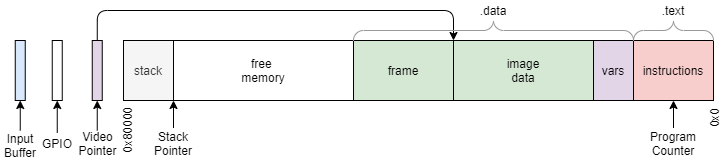
\includegraphics[width=\textwidth]{emulator memory}

\subparagraph*{Stack}
Pre-indexing with base register alteration, and branches with linking work, allowing the assembled brl (branch link), ret, push and pop commands to function.
\subparagraph*{New Flags}
Added flags for \textbf{-v} (video output, keyboard input on), \textbf{-n} (do not display memory), \textbf{-g} (show GPIO bits), \textbf{-h} show help menu. The register output has also been updated to show the \textbf{SP} and \textbf{LR} registers.
\subparagraph*{Display}
By passing the \textbf{-v} flag the emulator will display the memory region starting at the pointer contained in special location (0x1000000 - the video pointer) at a fixed resolution (192x108) with full RGB colour (4 bytes per pixel, ABGR format). When a value is stored to the memory pointer, the display is updated.
\newline\newline We used the SDL2 graphics library to render a texture, which used the data stored at the memory pointer (a part of the addressable emulator memory). The graphics are scaled up by 4 as on newer monitors the window would be too small to play PONG.
\newline\newline Reading texture data directly from the emulator memory proved to be much faster than iterating through the all pixels, rendering. Though this meant that each pixel had a redundant byte (alpha value) associated.
\subparagraph{Keyboard Input}
When the video output is on, input keystrokes are taken and written to a buffer. To access this buffer the program being run must access the input buffer at memory location (0x3000000), which will contain the next character. By storing 0 to this location, the buffer is cleared, and the emulator will place the next key pressed in the location.
\begin{center}
	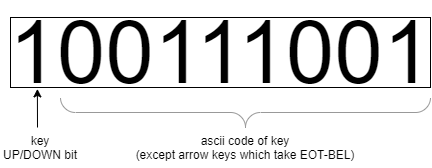
\includegraphics[scale = 0.5]{emulator keyboard input}
\end{center}
\subparagraph*{Testing}
To test the graphics and keyboard input, we created a small python program to convert an image's black pixels into an ARM subroutine to draw pixels. This was then used to create a a test program, with flashing text and that responded to a space key press to change the display.
We changed the input buffer from a cyclical array queue in emulator memory, to a special memory location to simplify the arm code and fix issues with input in response to the tests.
\centerline{\textbf{Initial Test program for Emulator Keyboard Input and Graphics}}
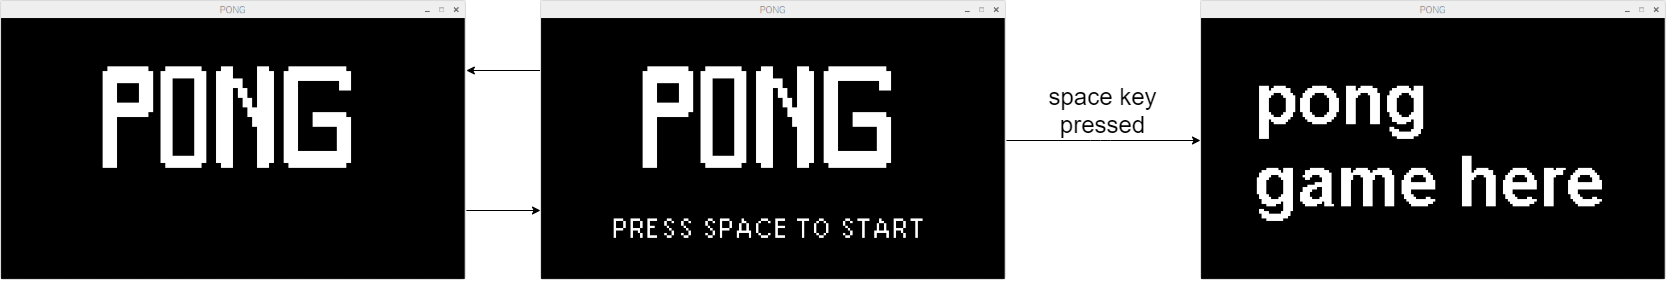
\includegraphics[width = \textwidth]{emulator testing PONG program}
For the final program, to reduce draw time for complex graphics, we made use of the .data region of the program to store image data ready to display. This data was generated by a bmp to ARM .data section file converter built in python.
\subsection*{Pong}
\begin{center}
	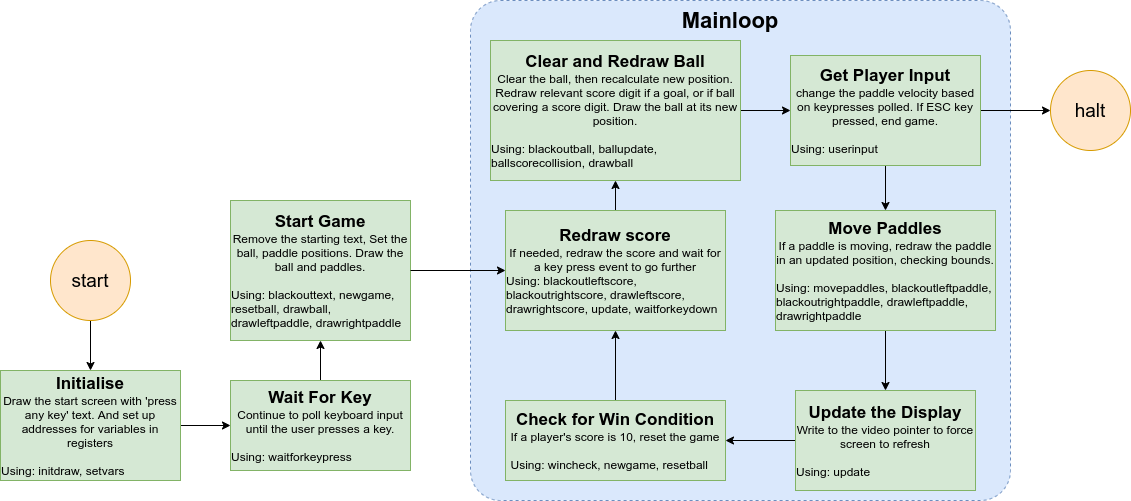
\includegraphics[width = \textwidth]{pong game structure}\\
\end{center}
\begin{center}
	\begin{tabular}{l|c|r}
		\textbf{Section} & \textbf{Purpose} & \textbf{Assigned to}\\
		Mainloop & The main loop of the program. Updating display, checking win conditions. & Oliver\\
		Initialise & Draws the initial page of the pong game. & Bartek \& Ioana\\
		Draw & Independent subroutines to draw ball, paddles, digits for score. & Bartek \& Ioana\\
		Blackout & Removes the old instances of screen elements. & Bartek \& Ioana\\
		Ball Update & Performs collision detection, changing ball position and velocity as well as score. & Jordan \& Ioana\\
		User Input & Takes input from buffer provided by emulator and moves paddles accordingly. & Oliver \\
	\end{tabular}
\end{center}

\centerline{\textbf{INSERT PICTURES OF PONG GAME HERE}}
\section{Group Reflection}
\subsection*{Communication}
In order to keep a high level of information synchronization between the team members, we used the following techniques:
\begin{itemize}
\item \textbf{Meetings:}\\
Our team held at least 2 meetings per week to discuss the progress with the task, the technical difficulties that might had arisen and the goals of the next sprint (as in the SCRUM team project methodology). Furthermore, summaries have been compiled after each meeting to allow to easily refer to the contents of the meeting when needed. 
\item \textbf{Pair communication:}\\
Apart from our meetings, we kept a higher throughput of communication in pairs to allow for easy and quick resolution of any problems in more than one area of development. For that reason, some of our in-pair meetings were held in person, especially in the groups that developed the assembler and emulator.
\end{itemize}
\subsection*{Individual Reflections}

\subparagraph*{Jordan}
During the course of this project, I made a great effort to integrate well with my team mates. From my group feedback and continuous feedback from my colleagues, I believe I fitted in with my team mates considerably well. As a result, group communication between myself and my team mates was smooth and effective, and I enjoyed working with my team.
\subparagraph*{Ioana}
This project has been a great opportunity to improve myself. I learnt how to write cleaner code, how to document it properly, and also how to divide complex problems into manageable tasks. Unlike some of my teammates, I had no prior experience with graphics or compilers, but I made a genuine effort and picked up the pace quite fast. I think one of my biggest strengths has been my communication skills: whenever I didn't understand something, I asked, whenever I thought I could handle a task, I claimed it. I enjoyed working on this project a lot, I'm proud of our end result, and I'm grateful for what I learnt from my teammates.
\subparagraph*{Oliver}
I was more than satisfied with the level of performance and cleanliness of my code. The emulator is fast, reliable and the extension doubly so. While I had done C before, it was never to this standard and I am happy to say I have learnt a lot, not just about writing good C, but also in project structure/build, git repo management, graphics as well as making the best use of, and being the best use to, my teammates. One thing I would improve with more time would be profiling done on the emulator, we had limited success getting analysis through gprof (make profile in src/emulate) and with more time I'm sure we could improve speed (especially on lower spec devices such as the pi, with graphics).
\subparagraph*{Bartek}
I believe I did everything I could as far as this project goes. My code looks fairly clean, my testing is as robust as I could have made it provided this amount of time and the optimizations are as good as they could have been in C. Also, I was able to trust my teammates with the code more than I did in all my past projects. The only things that I would change is a better work life ballance, learn a different collaborative coding style (the only one I know is to split the workload into non-overlaping sections with known interfaces) and improve my git workflow to make it a bit cleaner.
\end{document}